\documentclass{article}
\usepackage{amsmath}
\usepackage{pgfplots}
\usepackage{graphicx}
\usepackage{enumitem}
\usepackage{hyperref}
\usepackage{fancyhdr}
\pagestyle{fancy}
\lhead{Notes by Tianyu Du}
\usepackage[
	type={CC},
	modifier={by-nc-sa},
	version={3.0},
]
{doclicense}
\title{Chapter9 and Chapter10 on Tophat}
\author{Tianyu Du}
\date{\today}
\begin{document}
	\maketitle
	\doclicenseThis
	\tableofcontents
	\section{Chapter.7 Learning}
	\paragraph{Learning} involves a relatively permanent change in one's mental processes or behaviour that is a function of interactions with the environment. \emph{Learning and cortical development are optimal when the person is exposed to highly enriched environment.}
	\subsection{Pavlovian Conditioning}
	\paragraph{Classical conditioning}
	\paragraph{} Used concepts of \textbf{stimulus} and \textbf{response}, where stimulus can be anything in the environment that is measurable and evoke a response.
	\paragraph{} An \textbf{unconditional stimulus} causes an \textbf{unconditional response}.
	\paragraph{} A \textbf{neutral stimulus} is repeatedly paired with an unconditional stimulus so that the neutral stimulus becomes a \textbf{conditional stimulus}.
	\paragraph{} To create classical conditioning, Pavlov selected a neutral stimulus and paired it with an unconditional stimulus, which reflexively triggered an unconditional response.
	\paragraph{Reflexes} are \emph{involuntary} responses that are triggered or \textbf{elicited} by an \textbf{environmental event} that precedes and causes the \textbf{response} or \textbf{action}.
	\paragraph{Conclusion} The organism learns to do an involuntary reflexive response to a new, formerly neutral stimulus.
	\paragraph{Extinction} if the conditional stimulus is presented without the unconditional stimulus, the strength of conditional response decreases over time.
	\paragraph{Spontaneous recovery} of the conditional response occurs if the extinguished conditional stimulus is again presented.
	\subsubsection{Associating Stimuli}
	\begin{itemize}
		\item Start the pairing with the neutral stimulus presented first before the unconditional stimulus.
		\begin{itemize}
			\item Short-delay.
			\item Long-delay.
			\item Trace conditioning.
		\end{itemize}
		\item Simultaneous conditioning.
		\item Backward conditioning. (UCS comes before NS/CS)
	\end{itemize}
	\begin{figure*}
		\centering
		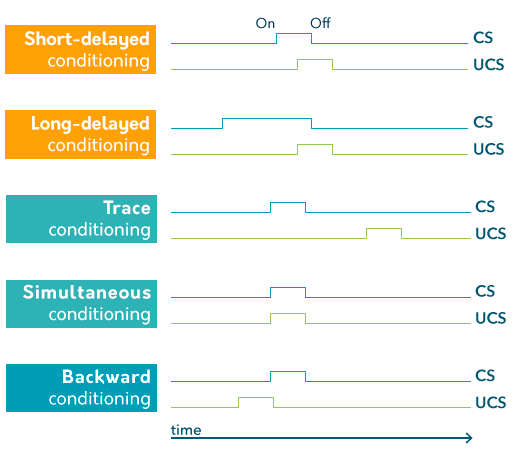
\includegraphics[width = \linewidth]{pic/conditioning_methods}
		\caption{Five types of temporal conditioning procedures.}
	\end{figure*}
	\paragraph{}\textbf{The most effective pairing methods occur when the conditional stimulus precedes the unconditional stimulus.}
	\paragraph{} \emph{Animals don't care about the conditional stimulus; it's the unconditional stimulus and its temporal relationship with the conditional stimulus that is important}.
	\paragraph{Aversive stimulus} stimulus that is conditioned with unpleasant consequence.
	\subsection{How is Pavlovian Conditioning Related to "What We Do"}
	\paragraph{Appetitive Unconditional Stimulus} Involving something pleasant.
	\paragraph{Aversive Unconditional Stimulus} Involving some degree of physical discomfort.
	\paragraph{Example} If a new product is paired repeatedly with an actor we respect and like, Pavlovian conditioning would suggest that we will associate our liking of the actor to the product.
	\subsection{Other Principles associated with Classical Conditioning}
	\paragraph{Stimulus Generalization} involves reacting in a similar manner to stimulus \emph{share features} associated with the original condition stimulus.
	\paragraph{Stimulus Discrimination} with stimulus discrimination, conditional responses \emph{only} when the original conditional stimulus is introduced. \underbar{Similar stimuli do not elicit a response.}
	\paragraph{Higher order conditioning} pavlovian conditioning can also occur when a \textbf{neutral stimulus} is systematically and repeatedly paired with an \textbf{existing conditional stimulus}.
	\paragraph{Biological preparedness} makes it easier to condition fear to snakes and spiders than to arbitrary stimuli like a flower and a tone.
	
	\textbf{Implication: phobias}: \textbf{Phobias} are often different from fear conditioning in the laboratory, because phobias:
	\begin{enumerate}
		\item are easily acquired in a single trial.
		\item can persist even when the person knows that the feared object is incapable of harm.
		\item are of things that could harm our ancestors but are far less prevalent in today's world.
		\item do not extinguish quickly or easily.
	\end{enumerate}
	\subsection{Development of the Behavioural Perspective and "Little Albert"}
	\paragraph{John B. Watson} American psychologist.
	\paragraph{Behaviourism} is the perspective within psychology that focuses on the \textbf{acquisition} and \textbf{modification} of an organism's behavioural responses.
	\subsection{Operant Conditioning}
	\paragraph{E.L. Thorndike} American psychologist.s
	\paragraph{} Also called \textbf{instrumental conditioning}.
	\paragraph{Law of effect}
	\begin{itemize}
		\item Behaviours that yielded satisfying consequences are more likely to recur.
		\item Behaviours that result in discomfort are less likely to be repeated.
	\end{itemize}
	\paragraph{} Focus on how the \textbf{consequences} of \emph{voluntary behaviour} influence subsequent behaviour.
	\paragraph{B.F. Skinner} Importance of the environmental events that preceded behaviour. (\textbf{antecedent stimuli}).
	\paragraph{Lindsley: Dead man's test} if a dead man can do it, then it isn't behaviour.
	\paragraph{Skinner} people and nonhumans learn about the environmental events(antecedents and consequences) that affect their behaviour.
	\paragraph{4 Contingencies} between responses and their consequences to describe these situations so that we can predict future behaviour.
	\begin{enumerate}
		\item \textbf{Reinforcement} the consequence of a response \emph{increase the probability} of behaviour.
		\item \textbf{Punishment} \emph{decrease the likelihood} of a recurrence of a behaviour.
	\end{enumerate}
	\begin{enumerate}
		\item \textbf{Positive} the application or the addition of something.
		\item \textbf{Negative} removal of something from the environment.
	\end{enumerate}
	\begin{figure*}
		\centering
		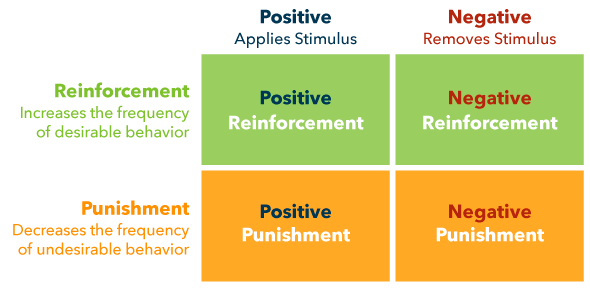
\includegraphics[width = \linewidth]{pic/reinforcing_types}
		\caption{Types of effects on sub-sequential likelihood of behaviour.}
	\end{figure*}
	\paragraph{} In these analyzed situations, we assume that the response \emph{always} occurs, but what we don't know about it what will happen in the consequence.
	\paragraph{} If we're talking about a positive contingency, then both the response and the consequence occur. If we're talking about a negative contingency, then the response occurs but the consequence is that it (the environmental event) is removed or avoided.
	\paragraph{Analyze contingency}
	\begin{enumerate}
		\item Identify the response or \textbf{target behaviour}.
		\item Identify the \textbf{consequence}.
		\item Identify the \textbf{addition or removal} of consequence.
		\item Identify the \textbf{change in likelihood} of future occurrence.
	\end{enumerate}
	\paragraph{Extinction} is \textbf{not} a contingency in and of itself. It's actually the absence of a contingency.
	\subsubsection{Escape and Avoidance}
	\paragraph{Escape} is a situation in which the aversive stimulus is already present and a response removes or stops the otherwise ongoing aversive stimulus.
	\paragraph{Avoidance} is a situation in which the aversive stimulus is not currently present but will occur unless you emit a response to cancel the scheduled aversive event. And is sometimes called \textbf{active avoidance}.
	\paragraph{} When punishment is used by itself, the organism is only learning \emph{what not to do} rather than what responses it should be doing instead. People who employ punishment are being negatively reinforced to do so because it decreases the response the person does not like (\emph{the negative reinforcer}).
	\subsubsection{Extinction} 
	\paragraph{Extinction} a response used to produce a consequence, but that consequence is no longer provided.
	
	\textbf{Behavioural effects of extinction}
	\begin{itemize}
		\item Temporary increase in responding, \textbf{extinction burst}.
		\item Emotional and aggressive responding.
		\item Responding eventually stops.
	\end{itemize}
	
	We know that extinction eventually decreases behaviour, but how quickly it decreases behaviour depends upon how regularly the consequence was delivered.
	\paragraph{Partial reinforcement extinction effect} Behaviour exposed to a \emph{continuous reinforcement schedule} will extinguish \emph{faster} in extinction than behaviour exposed to an \emph{intermittent reinforcement schedule}.
	\subsection{Reinforcers}
	\paragraph{Reinforcers} are events or stimuli that follow behaviour and \emph{increase the future likelihood} of that kind of response.
	
	Reinforcers are called \textbf{positive} if they strengthen \emph{responses they follow}; they are \textbf{negative} if they strengthen responses that \emph{lead to their removal}.
	
	\paragraph{Primary(or unconditioned) reinforcers} are \textbf{not} learned; they naturally affect responses they follow. \emph{Primary positive reinforcers} generally are stimuli/events needed to maintain life. \emph{Primary negative reinforcers} typically include aversive events such as heat and pain. Primary reinforcers tend to be involved in those contingencies proved by natural environment.
	
	\paragraph{Secondary(or conditioned) reinforcers}, both positive and negative, acquire their capacity to affect responses they follow because they have been associated or paired with \emph{primary} or \emph{already-conditioned secondary reinforcers}.(higher order conditioning.)
	
	\subsubsection{Using Consequences Effectively}
	\paragraph{Factors influence the effectiveness of the impact of reinforcers on responses.}
	\begin{itemize}
		\item \textbf{Immediacy} means that there must \textbf{not} be a much of a delay between the occurrence of the response and the occurrence of the consequence.
		\item \textbf{Power} is the idea that the reinforcer must be strong enough to influence the response.
		\item \textbf{Contingency} requires that there must be an \textbf{if-then} relationship between the response and the consequence.
		\item \textbf{Instruction} explanation ti the person what the contingency involves.
	\end{itemize}
	\paragraph{Premack's Principle of Reinforcer Efficacy} is based on how often behaviours occur. If behaviour A occurs more frequently than behaviour B, access to behaviour A can be made contingent on \textbf{first doing behaviour B}.
	\subsection{Scheduling Consequences}
	\paragraph{Schedules of reinforcement}
	\subsubsection{Ratio Reinforcement Schedules}
	\paragraph{} Schedules of reinforcement fall into two categories, \textbf{ratio} and \textbf{interval}, and each category has two sub-divisions, \textbf{fixed} and \textbf{variable}.
	\paragraph{FR(n)}: requires n times of target response for one reinforcer to occur.
	\paragraph{FR(-1)}: \textbf{Continuous}
	\paragraph{VR(n)}: the number of times that targeted response much occur changes around a mean average n.
	\begin{figure*}
		\centering
		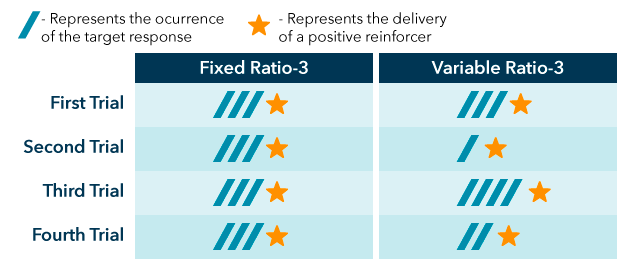
\includegraphics[width=\linewidth]{pic/reinforce_ratio}
		\caption{Required number of responses to trigger reinforcement for FR-3 compared to a VR-3 schedule.}
	\end{figure*}
	\subsubsection{Interval Reinforcement Schedules}
	\paragraph{Interval schedules} require that a specific amount of \emph{time elapse} before an occurrence of targeted response will trigger the delivery of a positive reinforcer.
	\paragraph{FI-n min} \textbf{None} of the targeted responses that occur during the one-minute interval are reinforced.
	\begin{figure*}
		\centering
		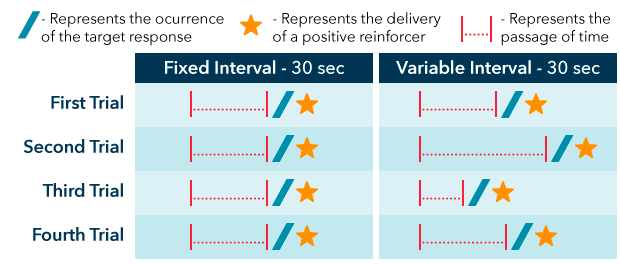
\includegraphics[width = \linewidth ]{pic/reinforcing_interval}
		\caption{Required number of responses to trigger reinforcement for a FI-30 sec and a VI-30 sec schedule}
	\end{figure*}
	\subsubsection{Operant Stimulus Discrimination}
	\paragraph{Discriminative stimulus} the antecedent stimulus in operant conditioning, if it affects the likelihood of the response occurring.
	\paragraph{} Positive reinforcement is used to:
	\begin{itemize}
		\item Maintain a response at its current level.
		\item Increase a response over its current level.
		\item Teach new responses to the organism. (\textbf{shaping})
	\end{itemize}
	\subsubsection{Comparing Pavlovian to Operant Conditioning}
	\paragraph{Pavlovian Conditioning} involving unconditional stimulus.
	\paragraph{Operant Conditioning} involving reinforcer/punisher.
	\paragraph{Operant Conditioning} the response \textbf{does} change the probability of the consequence.
	\paragraph{Pavlovian Conditioning} affects involuntary behaviours.
	\paragraph{Operant Conditioning} involves voluntary responses.
	\paragraph{Pavlovian Conditioning} a new stimulus (the conditional stimulus) evokes a response that the organism is \textbf{already capable} of performing.
	\subsection{Tolman's Latent Learning}
	\subsubsection{Social Learning}
	\paragraph{} The children who had observed the adults \textbf{modelled} what they saw the adults do.
	\paragraph{Vicarious learning} watching another person act, including any consequences the acting person experiences, can indirectly (vicariously) reinforce that action in the learner when she finds herself in a similar situation.
	\paragraph{Four phases/processes/stages of observational learning}
	\begin{enumerate}
		\item \textbf{Attentional phase} the learner must notice the behaviours being modelled.
		\item \textbf{Retention phase} the learner covertly practices and encodes the performance being observed.
		\item \textbf{Production phase} the learner \textbf{imitates} the behaviour observed.
		\item \textbf{Motivational phase} the imitated performance is likely to trigger similar types of consequences (positive or negative) that may or may not have been during the attentional phase.
	\end{enumerate}
	\subsection{Biological Constraints on Learning and Learned Helplessness}
	\paragraph{Biological constraints} how a species' characteristics, often genetic, can affect learning in that some responses and associations are more easily learned and others.
	\paragraph{Learned helplessness} when the organism's escape responses are ineffective at decreasing the painful events being experience, the escape and avoidance responses eventually stop.

	\section{Chapter.8 Memory}
	\subsection{Introduction}
	\subsubsection{Metaphors for Memory}
	\paragraph{Plato and Aristotle} described memory as a \emph{wax tablet}. Experiences pressed into the tablet, creating shapes and patterns of writing. 
	\paragraph{Failure of search} inability to remember something.
	\paragraph{Reconstruction} is a better metaphor because rather than specifically searching for information, you create a useful response given the situation at hand and what you've stored.

	\subsection{Encoding Memories: Prolonging the Present}
	\paragraph{Encoding} how our brains commit an event to memory. The problem our brains have to solve in order to encode information is called the \textbf{encoding problem}.
	\paragraph{Storing} memories are stored as part of brain's physical structure. Correlated to \textbf{storage problem}
	\subsubsection{Sensory Memory: Icons and Echoes}
	\paragraph{} \emph{Sensory memory is a system that keeps information translated by the senses briefly active in a relative \textbf{unaltered}, \textbf{unexamined} form.}
	\paragraph{Iconic memory} In the \textbf{visual} system.
	\paragraph{Echoic memory} In the \textbf{auditory} system. \emph{Echoes have been demonstrated to last longer}.
	\subsubsection{Immediate Memory: Manipulating Information}
	\paragraph{Immediate memory} is the system that actively holds information at the \textbf{front} of your mind. Also referred as \emph{short-term} or \emph{working} memory
	\paragraph{Characteristics of Immediate Memory}
	\begin{itemize}
		\item \textbf{Representation}
		\begin{itemize}
			\item \textbf{Inner voice} is evidence that information in immediate memory can be represented \textbf{verbally}. \emph{the primary mode of coding information in immediate memory is believed to be auditory.}
			\item \textbf{Inner eye} visual coding.
		\end{itemize}
		\item \textbf{Duration} Information can be stored in immediate memory for \textbf{forever}. But, \textbf{rehearsal} is required.
		\item \textbf{Capacity} the average person could hold about seven separate pieces of information at a time in their mind. Called \textbf{memory span}. \textbf{Chunking} is potentially a route to improve the capacity of immediate memory.
	\end{itemize}
	
	\paragraph{The working memory model} immediate memory is not simply a place for the storage of information, but primarily a place for the \emph{manipulation of information}.
	\begin{itemize}
		\item \textbf{Phonological loop} is where \textbf{auditory} and \textbf{verbal} information is temporarily stored and manipulated.	
		\item \textbf{Visuospatial sketchpad} is the representation of inner eye in the model, and represents a place where \textbf{visual} and \textbf{spatial} information is stored and manipulated.
	\end{itemize}
	\paragraph{Central executive} to direct the flow of information to and from the phonological loop, the visuospatial sketchpad and \textbf{long-term memory}.
	\subsection{Long-Term Memory: Connection \& Storage}
	\subsubsection{Kinds of Long-term Memory}
	\paragraph{Episodic memories} auto-biographical memories that are based on life events and all about \textbf{specific context}.
	\paragraph{Semantic memories} relate to \textbf{meaning devoid} of a specific context.
	\paragraph{Procedural memories}
	\subsubsection{The Transfer to Long-term Memory}
	\paragraph{Elaborative rehearsal} refers to a process of \textbf{actively manipulating} information in \emph{immediate memory} so that we can \textbf{meaningfully connect} it to other information that we've already stored in long-term memory.
	\paragraph{Deep processing} making meaningful connections to \textbf{existing knowledge}.
	\paragraph{Shallow processing} encoding information based on only its \textbf{surface characteristics}.
	\begin{figure*}
		\centering
		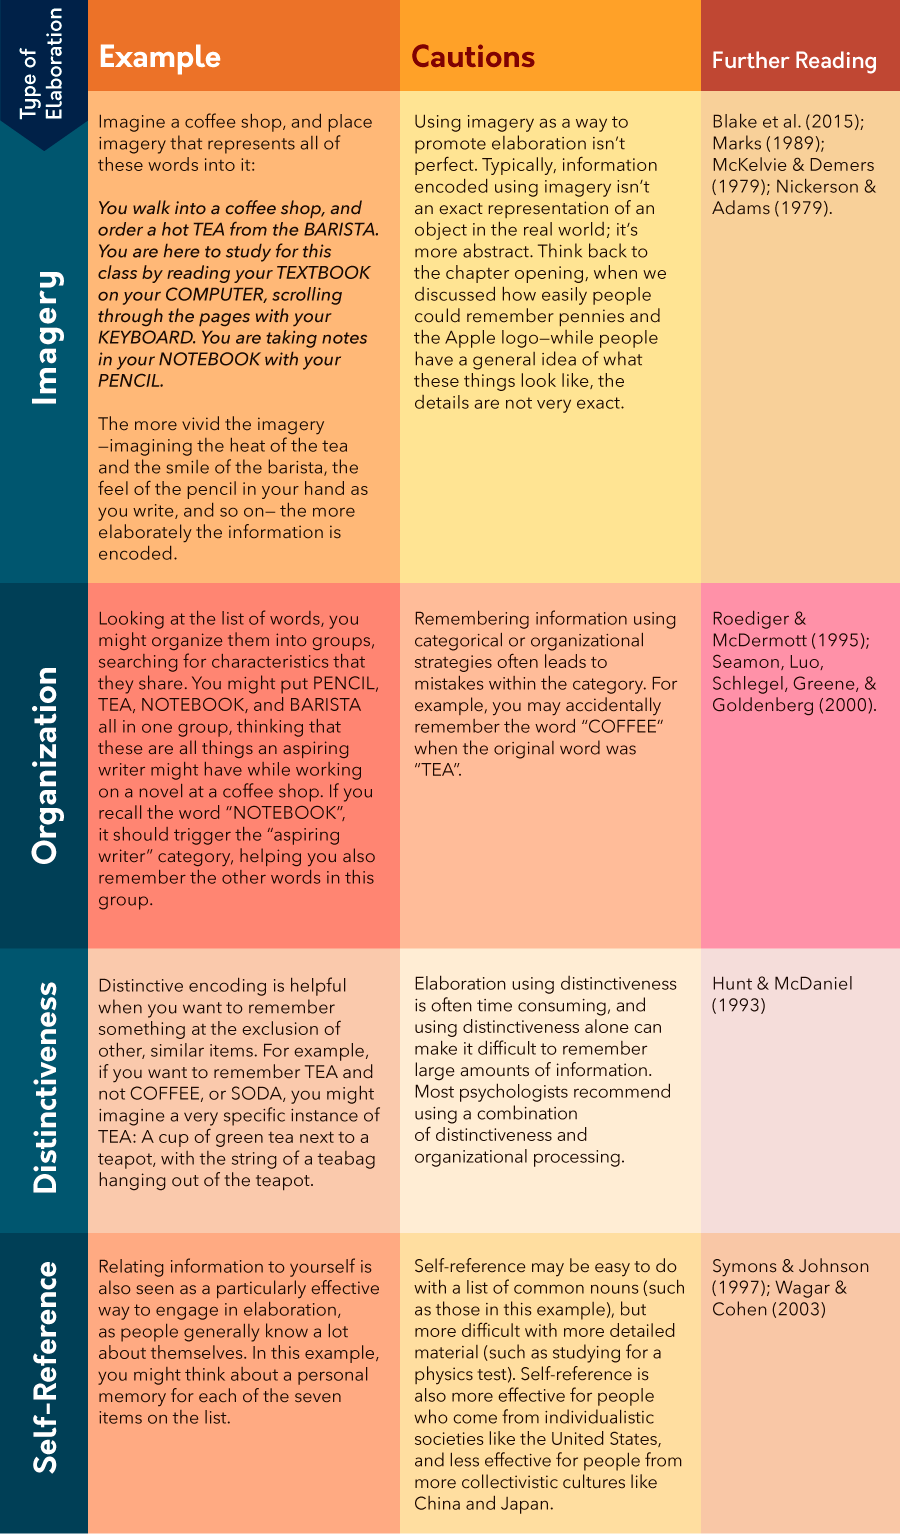
\includegraphics[width = \linewidth]{pic/elaboration_types}
		\caption{Types of Elaboration}
	\end{figure*}
	\subsubsection{Effective Encoding Strategies}
	\paragraph{Massed practice} not effective.
	\paragraph{Spacing effect} spacing out your studying over multiple hours, days, weeks, or months is the key to long-term learning.
	\paragraph{Mnemonics} work by providing a \textbf{framework} for your engage in the kind of meaningful processing.
	\paragraph{Mind palace}
	\paragraph{Retrieval practice}
	\subsection{Memory Retrieval}
	\paragraph{Cues} are pieces of information in the present that help us remember events from the past, and they are central to remembering.
	\begin{itemize}
		\item \textbf{Free recall}
		\item \textbf{Cued recall}
	\end{itemize}
	\paragraph{The Encoding Specificity Principle} a natural consequence of the importance of cues is that how we encode information affects how we are able to retrieve it.
	\paragraph{}\emph{\textbf{Context at encoding matters.}}
	\paragraph{Transfer-Appropriate Processing} we should \textbf{not} only attempt to match the context that occurs at both encoding and retrieval, but also, we gotta attempt to match the \emph{physical} and \emph{mental} processes that are occurring.
	\subsubsection{Implicit Memory}
	\paragraph{Implicit memory} we remember information without consciously realizing or intending it.
	
	\emph{the kinds of elaborative encoding strategies that facilitate explicit remembering often have no effect on implicit memory}.
	
	\subsection{Memory Errors and the Process of Forgetting}
	\subsubsection{Memory Errors}
	\paragraph{Seven sins of memory}
	\begin{enumerate}
		\item \textbf{Errors of omission} information cannot be brought to mind.
			\begin{itemize}
				\item \textbf{Transience} describes how memory for any particular event or piece of information tends to \emph{degrade} over time, often simply called \emph{forgetting}.
				\item \textbf{Decay}.
				\item \textbf{Retroactive interference} \emph{newly learned information} makes it more difficult to recall older information.
				\item \textbf{Proactive interference} when \emph{old information} interferences with new information.
				\item \textbf{absent-mindedness} when information is not encoded to begin with, whether due to attention or a failure to elaborately rehearse the information.
				\item \textbf{Blocking} relates to whether the cues we have available are enough to help us remember a piece of information.
				\item \textbf{Tip-of-the-tongue(TOT) state} when people cannot remember a piece of information, but have a powerful feeling that they know what they are trying to remember.
			\end{itemize}
		\item \textbf{Errors of commission} wrong or unwanted information is brought to mind. 
			\begin{itemize}
				\item \textbf{Misattribution} occurs when we incorrectly recall the source of information we are trying to remember. Also referred as \emph{Source errors}.
					\emph{\textbf{Déjà vu} we simply \underbar{cannot} remember the source of the information, rather than misattribute it.}
				\item \textbf{Flashbulb memories} are memories for events that are both \emph{surprising} and particularly \emph{significant}. \emph{These data suggest that for flashbulb memories, they aren't so much elaborately encoded as they are tinged with \textbf{emotion}}.
				\item \textbf{Suggestibility} suggestibility requires the information that is misremembered have been \emph{suggested by an \textbf{outside source}}. Example: \textbf{misinformation effect}.
				\item \textbf{Bias} most common: \textbf{schemas} are highly organized sets of facts and knowledge about specific kinds of information.
				\item \textbf{Persistence} occurs when the memory system fails to prevent the \emph{recall of memory that is unwanted}.
			\end{itemize}
		\item 
	\end{enumerate}
	\subsubsection{Forgetting and the Brain}
	\paragraph{Hyper-thymesia} leads to near perfect auto-biographical recall.
	\paragraph{Amnesia} any memory loss due to physical damage or problems in the brain.
	\begin{itemize}
		\item \textbf{Retrograde amnesia} forgetting everything pervious to the hit.
		\item \textbf{Anterograde amnesia} inability to make new memories.
	\end{itemize}
	
	\section{Chapter.9 Language \& thought}
	\subsection{Introduction}
	\paragraph{Greatest power of language} allowance for sharing and improving upon other's ideas.
	\paragraph{Productivity} Creation of new messages while speaking.
	\paragraph{} One import role of language is \textbf{social communication}
	\subsection{Development of Languages}
	\begin{itemize}
		\item \textbf{Tonal Language}: Rely on change in pitch to alter a word's \emph{meaning}. (e.g. Mandarin)
		\item \textbf{Intonation Language}: Primarily use pitch to convey \emph{feeling}. (e.g. English)
	\end{itemize}
	\paragraph{Implication} Children exposed to tonal languages become skilled at detecting [itch difference and are substantially more likely to exhibit perfect pitch compared to those exposed to intonation languages.
	\paragraph{Grammar and Syntax}
	\begin{itemize}
		\item \textbf{Grammar} (general) symmetric rules of a language.
		\item \textbf{Syntax} structure and consistent ordering of words.
	\end{itemize}

	\subsection{Theories on development}
	\paragraph{} B.F. Skinner argued that environmental influences strongly dictated language development, with Chomsky urged for the consideration of biological constraints on development.
	\subsubsection{B.F. Skinner: Nurture}
	\paragraph{Verbal Behaviour} Skinner defined speech as a \textbf{verbal behaviour}, and applied \textbf{operant conditioning} to languages acquisition. \emph{Otter factors reinforce children's language ability}.
	 
	\subsubsection{Noam Chomsky: Nativism}
	\paragraph{Nativism} the belief that certain abilities are built into our brains.
	\begin{itemize}
		\item \textbf{Critical Period}: 7 ~ 12 months. During this period, it is necessary for children to receive environmental stimulation in order to promote healthy development.
		\item \textbf{Sensitive Period}: \emph{Indicates that the neurological system is more malleable during early development but is still modifiable later in life with the proper environmental stimulation.}
	\end{itemize}
	
	\paragraph{Main pattens of languages}
	\begin{itemize}
		\item \textbf{SOV}: Subject-object-verb order.
		\item \textbf{SVO}: Subject-verb-object order.
	\end{itemize}

	\subsubsection{Emergentist perspective}
	\paragraph{} Development of language is the result of interaction among:
	\begin{enumerate}
		\item \textbf{Inherited biology} Explains development constraints.
		\item \textbf{Environmental factors}
		\item \textbf{Social Exposure} Explains individual differences and growth.
		\item \textbf{Behaviourist models(operant conditioning)} Provides predictions for how to modify verbal behaviours. 
	\end{enumerate}
	\paragraph{} A nativist approach would focus heavily on how an inherited speech bias and early flexibility prepare us to learn language, whereas an environmental perspective would emphasize that our development of speech is dependent on our exposure to, and familiarity with, our native language.
	\subsection{Language and Brain}
	\subsubsection{Broca's Aphasia / non-fluent aphasia}
	\paragraph{Example} Patient Tan. \emph{Initially appeared to have minimal head damage but soon worsened and was unable to produce speech.}
	\paragraph{} Linked to \textbf{Lower frontal lobe (Broca's Area)}.
	\paragraph{Founds}
	\begin{itemize}
		\item There may be a module in the brain controlling speech.
		\item \textbf{Hemispheric Lateralization} Language production is pre-dominantly controlled by the left hemisphere.
	\end{itemize}
	\subsubsection{Wennicke's Aphasia / fluent aphasia}
	\paragraph{} Wernicke's patient had damage to the temporal lobe and was still able to produce speech fluidly. However, the speech produced was not coherent.
	\paragraph{} Linked to \textbf{Temporal lobe (Wennicke's Area)}. \emph{Wernicke's area, and other areas of the temporal lobe, contribute to processing and differentiating understandable sounds from nonsensical noise. Being able to organize incoming auditory information and attach meaning is large apart of our language system.}
	\paragraph{} Ability to convey meaning is damaged.

	\subsection{Classifying words and objects}
	\paragraph{} \emph{Average human can produce 2~4 words per second and retrieve them from an impressive memory store of 50000 ~ 100000 words}.
	\paragraph{Mental Lexicon} information stored in Mental lexicon can be accessed within \emph{80 ms} and is organized by: 
	\begin{enumerate}
		\item \textbf{Phonemes}: smallest unit of sound information.
		\item \textbf{Morphemes}: smallest unit of language comprehension.
		\item The word is then quickly linked to other information that is \textbf{semantically} similar, or connected by the word's meaning. This \textbf{semantic network} of stored information allows us to put a word in context, retrieve relevant responses, and detect errors in usage.
	\end{enumerate}
	\paragraph{} \emph{The primary storage of conceptual knowledge is stored in our \textbf{left temporal lobe}}.

	\paragraph{Family Resemblance Theory} suggests that we classify the bird(objects) based on its \textbf{similarity} or \textbf{dissimilarity} to other members in our bird category.

	\paragraph{Prototype} is the most common or typical form a word assumes we imagine it.

	\paragraph{Sapir-Whorf Hypothesis / Linguistics Relativity} The structured differences in languages can alter one's perception and standing of reality. \emph{Reference of time and space differ based on cultural language patterns, and consequently can influence how we perceive time.}

	\subsection{Problem-Solving}
	\paragraph{} \emph{Problem-solving is commonly viewed as a sequential process involving this initial motivational state and the desired end-goal state}.
	\paragraph{Mental Set} \emph{Expectation of how to solve a problem} was influenced by their prior interaction and created a set effect, \textbf{fixedness}, limiting their application of new solution.

	\paragraph{Function Fixedness} Limiting us from using objects from purposes outside of their normal use.

	\paragraph{Strategy / Algorithm} An algorithm is a precise set of rules applied in order to solve a problem, and individual differences and environmental will dictate which algorithm we apply.

	\paragraph{Trail and Error} Commonly used when there are a limited number of available options. \emph{You can feasibly attempt a series of moves with little or no cost to yourself before finding the solution}.

	\paragraph{Heuristics} Used to help \emph{short-cut} the lengthy judgment and decision-making processes.
	\begin{enumerate}
		\item \emph{Example 1} \textbf{Mean-End Heuristics}: Positive reinforcement if state is moving towards goal state, and negative reinforcement if moving away from goal state.
		\item \emph{Example 2} \textbf{Representative Heuristics}: Mentally comparing something to our stored \textbf{prototype} of an event, object or person.
		\item \emph{Example 3} \textbf{Availability Heuristics}: We make judgment based on how easily instances of the same or related events are to retrieve from our memory, or how easily available those memories are. \emph{Analyze the \textbf{Frequency / Likelihood} of occurrence of event}.
	\end{enumerate}

	\paragraph{Steps of creative processes}
	\begin{enumerate}
		\item \textbf{Preparation} Gathering knowledge and proficiency with a topic.
		\item \textbf{Incubation} Requires the idea to sit on the back burner of your mind while you consciously work on something unrelated.
		\item \textbf{Illumination} To follow a period of \emph{slight pre-awareness}. (But is often reported to come as a surprise).
		\item \textbf{Evaluation} Evaluate your inspired idea and assess whether it is indeed, a creative and worthy solution.
	\end{enumerate}

	\subsection{Decision-Making}
	\paragraph{}\emph{We engage quick, short-cutting thinking that allow our minds to solve problems quickly. Although efficient, these shortcuts risk our decision making become \textbf{biased}, or systematically deviated based on our heuristics and judgment.}

	\paragraph{Confirmation Bias}: We have high tendency to seek out information that already confirms our ideas or beliefs. Additionally, with confirmation bias, information that is not consistent with one's existing beliefs is either ignored or distorted.

	\paragraph{Framing of options} Our choice and preferences are substantially altered based on the presentation or, framing, of options.

	\subsubsection{Dual process of decision making}
	\paragraph{Intuition} Reliance on \textbf{experience} and \textbf{emotions}.

	\begin{enumerate}
		\item \textbf{System 1: Intuitive decision} Making decisions based on \emph{quick, automatic} system. \emph{This system predominantly relies on emotional systems and stored experiences to guide thinking.}
		\item \textbf{System 2: Logical thinking} Counter commands those initial instincts. \emph{This system recruits thinking and reasoning areas of the brain}.
	\end{enumerate}

	\section{Chapter. 10 Intelligence}
	\paragraph{Defining Intelligence} \emph{Flynn}
	
	\emph{The word "intelligence" comes from two root words, inter, which means "between" and legere, which means "to choose, pick out, read". The original use of the word referred to the \textbf{ability to discern true or important information} from information that was false or unimportant. The root meaning of the word intelligence is similar to the modern expression of being able to read between the lines.}
	\subsection{Measuring Intelligence}

	\paragraph{Francis Galton} Focused on \textbf{physiological measures}.
	
	Focused on the empirical measurement of man using \textbf{empirical methods} to ensure precise measurement. Galton conceptualized that one's general cognitive ability (g) was the product of heredity, and he believed that the intelligence was related to how well one uses one's sense.
	\paragraph{Alfred Binet and Theodore Simion} Focused on \textbf{behavior} measures of intelligence on three aspects.
	\begin{enumerate}
		\item \textbf{Direction} Ability to know what to do and how to do it.
		\item \textbf{Adaptation} Ability to create strategies for implementing this knowledge and monitoring its progress.
		\item \textbf{Criticism} Ability to step back and find error in one's thinking.
	\end{enumerate}

	\paragraph{Lewis Terman: Stanford-Binet Test}: Based on Binet's work. Terman assumed that his test only measured intelligence and was not being affected by things such as language and cultural knowledge.
	\[
	IQ = \frac{\text{Mental Age}}{\text{Chronological Age}} * 100
	\]

	\textbf{Problem: } Inaccuracy after age of 16.

	\paragraph{David Wechsler: Deviation IQ}
	\begin{itemize}
		\item \textbf{Age in-dependency}: Solve the inaccuracy caused by age in Stanford-Binet test.
		\item \textbf{Point system} is used so that an individual does \textbf{not} have to answer a set number of questions in order to receive a score.
	\end{itemize}

	\subsection{Performance based measures of intelligence}
	\paragraph{Atkinson \& Shuffrin} Multi-Store Model of Memory.
	
	It explains the cognitive processing involved in memory, this model explained memory in terms of how information flowed between different types of processors (i.e. sensory, short-term, and long-term memory) and various methods of processing (i.e. selective attention, maintenance, and elaborative rehearsal).
	\begin{figure}
		\centering
		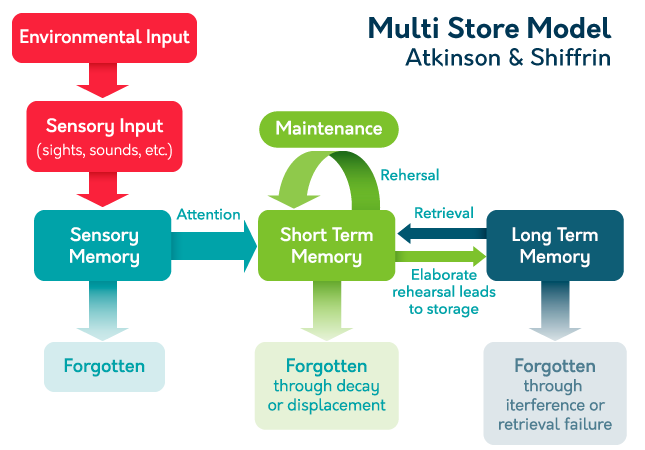
\includegraphics[width = \linewidth]{pic/Multi_store_model}
		\caption{Mult-Store Model of Memory.}
	\end{figure}
	
	\subsection{The use and misuse of intelligence testing}
	\paragraph{Example} Social Darwinism.
	\subsection{Problems with comparing the different groups}
	\paragraph{Stereotype threat} when people taking such (intelligence) tests, they feel pressure to \textbf{not provide} evidence supporting negative stereotypes of the group to which they belong.
	\paragraph{Mindset} A person's level of intelligence is part of that person's self-identity, which can ultimately affect a person's behaviour choices.
	\paragraph{Gender and Intelligence}
	\begin{itemize}
		\item Make: $\implies$ Visuospatial tasks.
		\item Female: $\implies$ Verbal tasks.
	\end{itemize}
	\subsection{The nature of intelligence: g and s}
	\paragraph{Spearman} initiated the use of \textbf{factor analysis} in the testing of intelligence. Factor analysis is the use of statistical measures to determine how much variable are related to each other in order to find clusters called "factors".
	\paragraph{g: general ability} This is a variable that stands for the general factor of intelligence, often simply called general intelligence or general cognitive abilities. Could be generalized across many different context.
	\paragraph{s: specific application} Contextually sensitive.
	\subsection{Raymond Cattell: Fluid intelligence and Crystallized intelligence}
	\paragraph{} \emph{Raymond Cattell(1971) tried to reconcile the \textbf{Spearman' theories} regrading \underbar{two levels of intelligence} with \textbf{Thurston's Theory} of \underbar{primary mental abilities,} which was comprised of two major factors found at the intermediary level: \textbf{fluid general intelligence(Gf)} and \textbf{crystallized general intelligence(Gc}.}
	\paragraph{Fluid intelligence} the ability to think flexible and to handle complex and novel situations. \emph{It is what you use to solve new problems that are not based primarily on knowledge you already process.}
	\paragraph{Crystallized intelligence} Ability to solve problems by applying previously accumulated knowledge.
	\paragraph{Cognitive Flexibility} Knowing how to apply one's knowledge.
	\begin{figure}
		\centering
		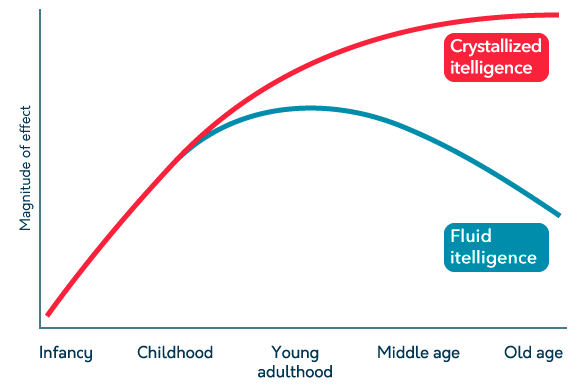
\includegraphics[width = \linewidth]{pic/fluid_and_crystallized_intelligences_over_ages}
		\caption{Fluid and crystallized intelligences across different stages.}	
	\end{figure}
	\paragraph{Wisdom Paradox} the fact that people seem to be able to become wiser even through many measures of cognitive functions show decline in later adult life.
	\subsection{Beyond the general intelligence}
	\paragraph{Emotional Intelligence (EI)} considers 4 components.
	\begin{enumerate}
		\item Ability to \textbf{perceive} emotion accurately.
		\item Ability to use emotions to \textbf{facilitate thought}.
		\item Ability to \textbf{understand} emotions.
		\item Ability to \textbf{manage} emotions.
	\end{enumerate}
	\paragraph{Stermberg's theory of Triarchic Intelligence}
	\begin{enumerate}
		\item \textbf{Analytical Intelligence} when the components are applied to the kinds of problems found in \emph{standard IQ tests}.
		\item \textbf{Creative Intelligence} when the components are applied to \emph{unfamiliar situations} where novelty is important.
		\item \textbf{Practical Intelligence} when the components are applied to \emph{real world settings}.
	\end{enumerate}
	
	Additionally, \textbf{successful intelligence}: the ability to appropriately use all these three intelligences so that one performs in the greatest possible variety of contexts.
	\paragraph{Howard Gardner's Multiple Intelligence} See Figure for details.
	\begin{figure}
		\centering
		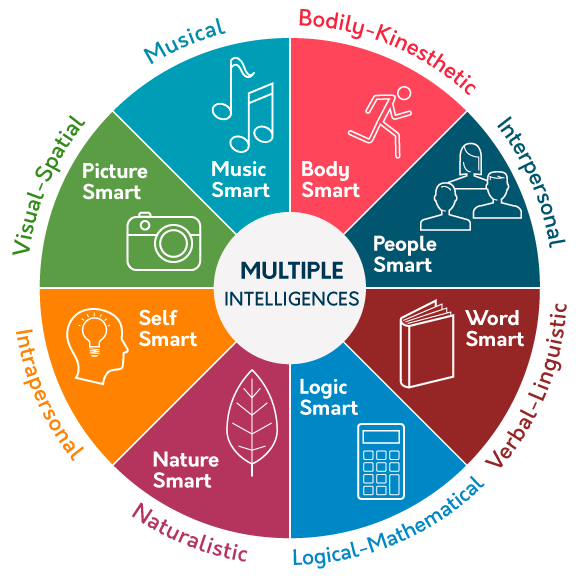
\includegraphics[width = \linewidth]{pic/multiple_intelligences}
		\caption{The Multiple Intelligence model by Howard Gardner}	
	\end{figure}
	\paragraph{Cultural Intelligence} Involving social learning abilities.
	\begin{itemize}
		\item Coordination of skills of attention.
		\item Working memory.
		\item Problem solving.
		\item Behavioural flexibility.
		\item Innovation.
	\end{itemize}
	\paragraph{Knowledge Illusion} Thinking we know more than we do, and understand more than we do.
	\subsection{The biology and culture of intelligence}
	\paragraph{} \textbf{Genetic}(nature) factors $\iff$ \textbf{Environmental} (nurture) factors.
\end{document}























